\documentclass[11pt]{article}
\usepackage[textwidth=18.0cm, textheight=23.0cm, top=2.0cm]{geometry}
\usepackage{pst-all}
\usepackage{amssymb}
\usepackage{tikz}
\usepackage{underscore}\begin{document}
\pagestyle{empty}


ClassName: \underline{\textbf{Class_08.2bp-12}}
\par
BinSize: \underline{\textbf{100 × 100}}
\par
ReduceSize: \underline{\textbf{100 × 100}}
\par
TypeNum: \underline{\textbf{40}}
\par
Num: \underline{\textbf{40}}
\par
OutS: \underline{\textbf{110000}}
\par
InS: \underline{\textbf{89243}}
\par
Rate: \underline{\textbf{0.811}}
\par
UB: \underline{\textbf{11}}
\par
LB0: \underline{\textbf{11}}
\par
LB: \underline{\textbf{11}}
\par
LBWithCut: \underline{\textbf{11}}
\par
NodeCut: \underline{\textbf{0}}
\par
ExtendedNodeCnt: \underline{\textbf{1}}
\par
GenNodeCnt: \underline{\textbf{1}}
\par
PrimalNode: \underline{\textbf{0}}
\par
ColumnCount: \underline{\textbf{11}}
\par
TotalCutCount: \underline{\textbf{0}}
\par
RootCutCount: \underline{\textbf{0}}
\par
LPSolverCnt: \underline{\textbf{1}}
\par
PricingSolverCnt: \underline{\textbf{0}}
\par
BranchAndBoundNum: \underline{\textbf{1}}
\par
isOpt: \underline{\textbf{true}}
\par
TimeOnInitSolution: \underline{\textbf{600.000 s}}
\par
TimeOnPrimal: \underline{\textbf{0.000 s}}
\par
TimeOnPricing: \underline{\textbf{0.000 s}}
\par
TimeOnRmp: \underline{\textbf{0.047 s}}
\par
TotalTime: \underline{\textbf{600.312 s}}
\par
\newpage


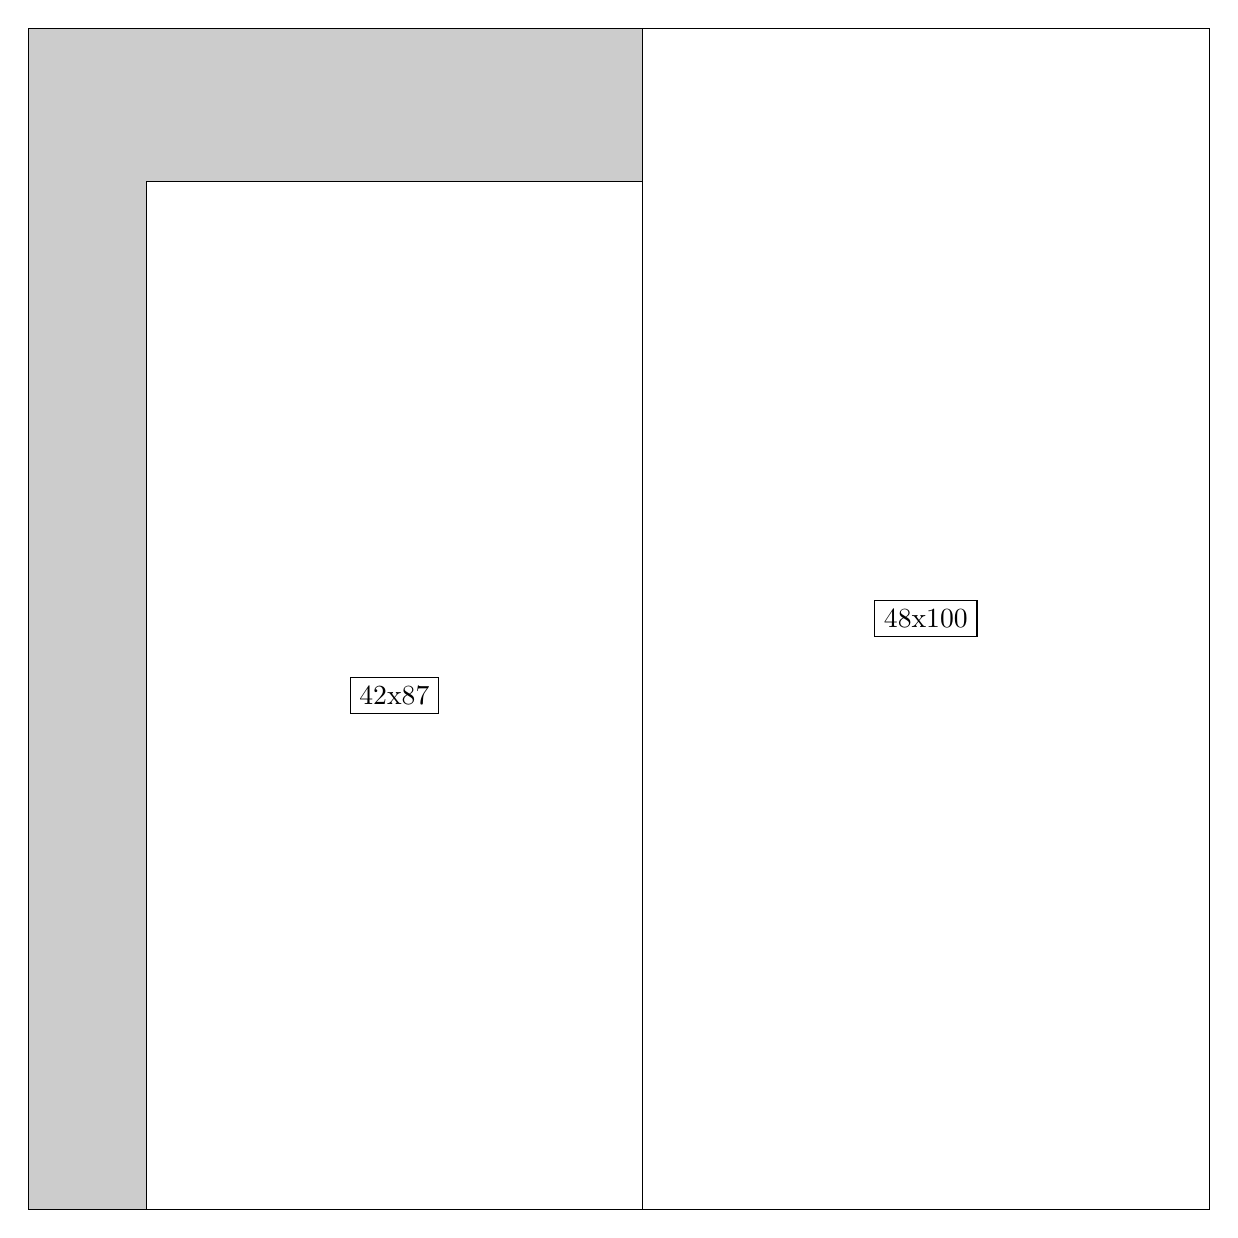
\begin{tikzpicture}[shorten >=1pt,scale=1.0,every node/.style={scale=1.0},->]
\tikzstyle{vertex}=[circle,fill=black!25,minimum size=14pt,inner sep=0pt]
\filldraw[fill=gray!40!white, draw=black] (0,0) rectangle (15.0,15.0);
\foreach \name/\x/\y/\w/\h in {48x100/7.8/0.0/7.199999999999999/15.0,42x87/1.5/0.0/6.3/13.049999999999999}
\filldraw[fill=white!40!white, draw=black] (\x,\y) rectangle node[draw] (\name) {\name} ++(\w,\h);
\end{tikzpicture}


w =48 , h =100 , x =52 , y =0 , v =4800
\par
w =42 , h =87 , x =10 , y =0 , v =3654
\par
\newpage


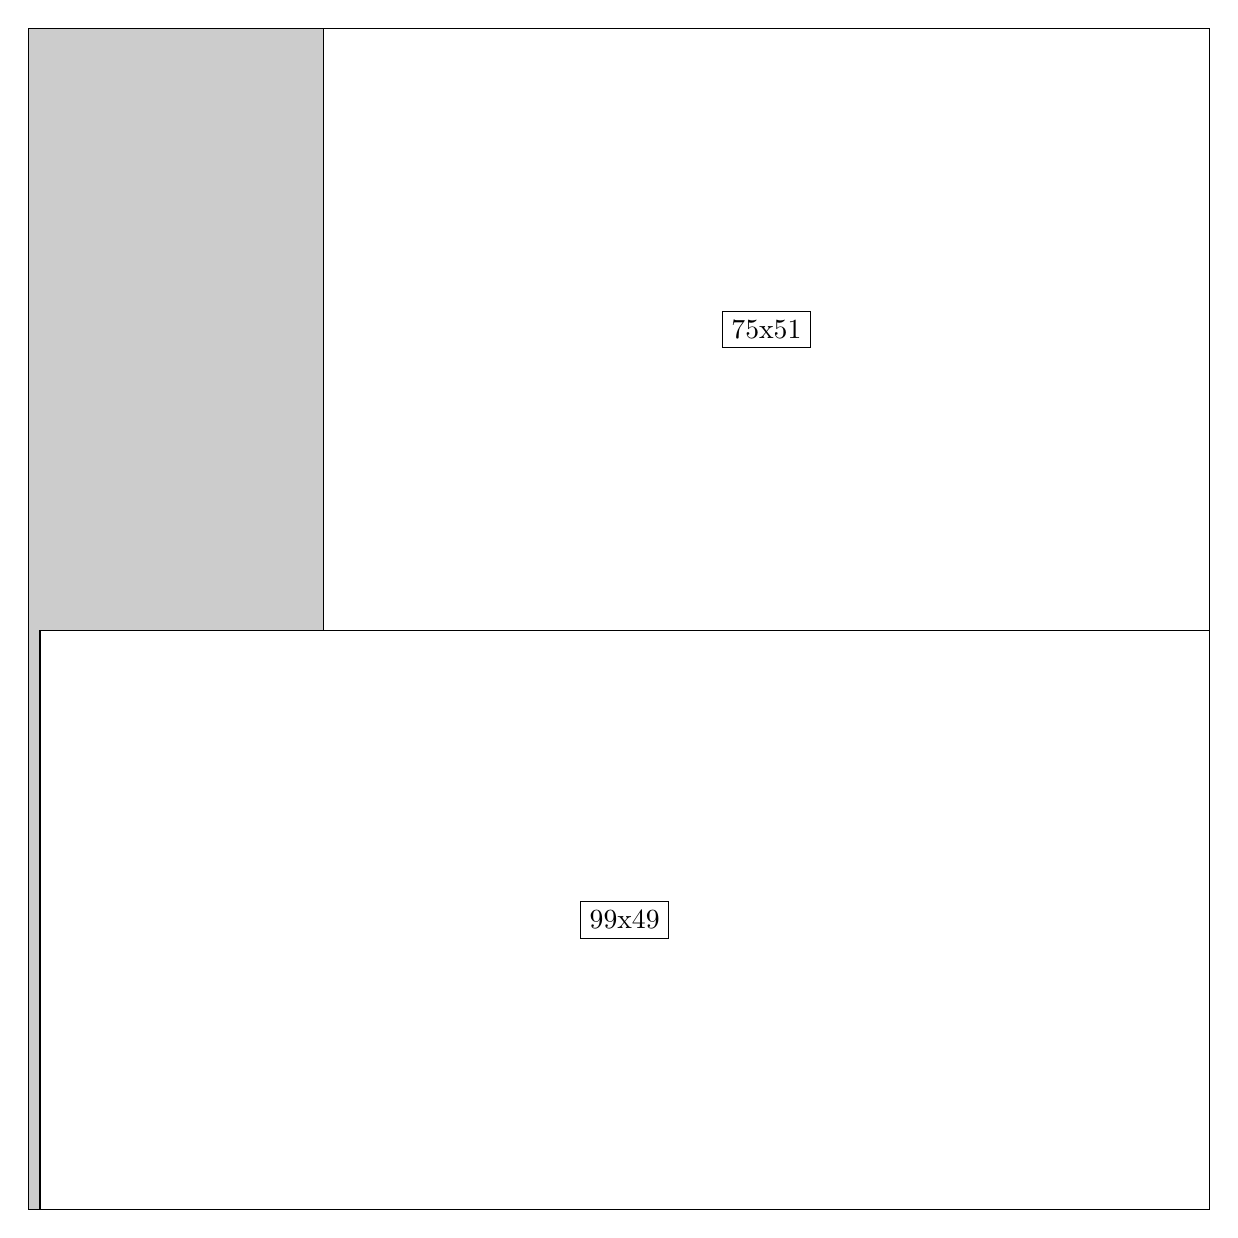
\begin{tikzpicture}[shorten >=1pt,scale=1.0,every node/.style={scale=1.0},->]
\tikzstyle{vertex}=[circle,fill=black!25,minimum size=14pt,inner sep=0pt]
\filldraw[fill=gray!40!white, draw=black] (0,0) rectangle (15.0,15.0);
\foreach \name/\x/\y/\w/\h in {99x49/0.15/0.0/14.85/7.35,75x51/3.75/7.35/11.25/7.6499999999999995}
\filldraw[fill=white!40!white, draw=black] (\x,\y) rectangle node[draw] (\name) {\name} ++(\w,\h);
\end{tikzpicture}


w =99 , h =49 , x =1 , y =0 , v =4851
\par
w =75 , h =51 , x =25 , y =49 , v =3825
\par
\newpage


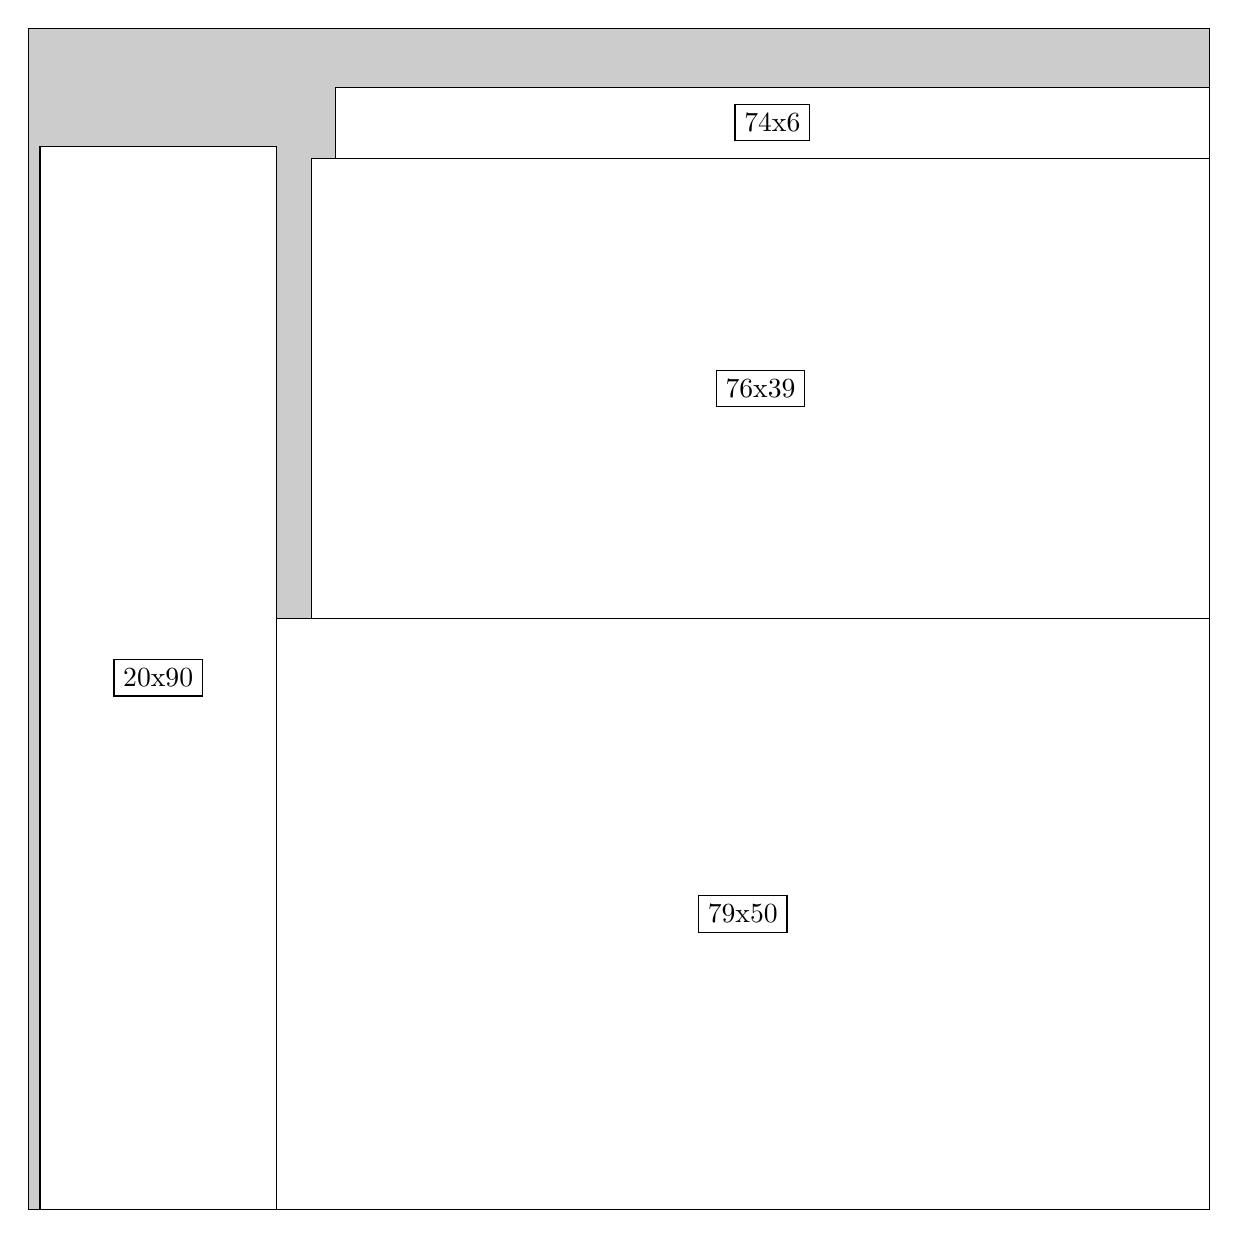
\begin{tikzpicture}[shorten >=1pt,scale=1.0,every node/.style={scale=1.0},->]
\tikzstyle{vertex}=[circle,fill=black!25,minimum size=14pt,inner sep=0pt]
\filldraw[fill=gray!40!white, draw=black] (0,0) rectangle (15.0,15.0);
\foreach \name/\x/\y/\w/\h in {79x50/3.15/0.0/11.85/7.5,76x39/3.5999999999999996/7.5/11.4/5.85,74x6/3.9/13.35/11.1/0.8999999999999999,20x90/0.15/0.0/3.0/13.5}
\filldraw[fill=white!40!white, draw=black] (\x,\y) rectangle node[draw] (\name) {\name} ++(\w,\h);
\end{tikzpicture}


w =79 , h =50 , x =21 , y =0 , v =3950
\par
w =76 , h =39 , x =24 , y =50 , v =2964
\par
w =74 , h =6 , x =26 , y =89 , v =444
\par
w =20 , h =90 , x =1 , y =0 , v =1800
\par
\newpage


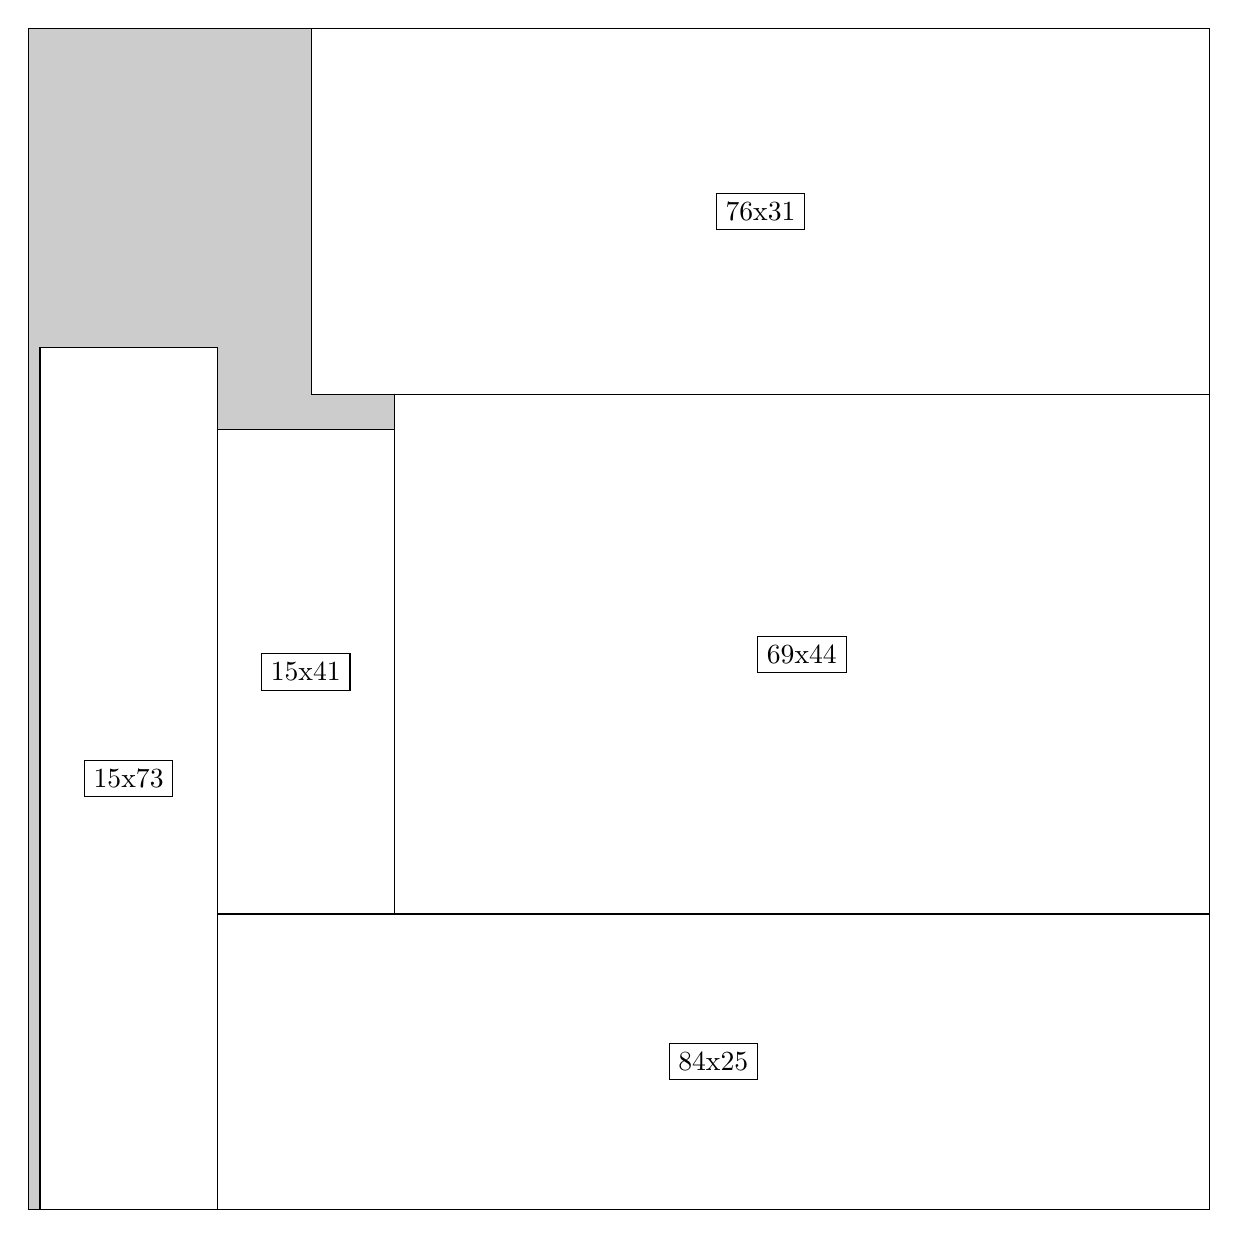
\begin{tikzpicture}[shorten >=1pt,scale=1.0,every node/.style={scale=1.0},->]
\tikzstyle{vertex}=[circle,fill=black!25,minimum size=14pt,inner sep=0pt]
\filldraw[fill=gray!40!white, draw=black] (0,0) rectangle (15.0,15.0);
\foreach \name/\x/\y/\w/\h in {84x25/2.4/0.0/12.6/3.75,69x44/4.6499999999999995/3.75/10.35/6.6,15x41/2.4/3.75/2.25/6.1499999999999995,76x31/3.5999999999999996/10.35/11.4/4.6499999999999995,15x73/0.15/0.0/2.25/10.95}
\filldraw[fill=white!40!white, draw=black] (\x,\y) rectangle node[draw] (\name) {\name} ++(\w,\h);
\end{tikzpicture}


w =84 , h =25 , x =16 , y =0 , v =2100
\par
w =69 , h =44 , x =31 , y =25 , v =3036
\par
w =15 , h =41 , x =16 , y =25 , v =615
\par
w =76 , h =31 , x =24 , y =69 , v =2356
\par
w =15 , h =73 , x =1 , y =0 , v =1095
\par
\newpage


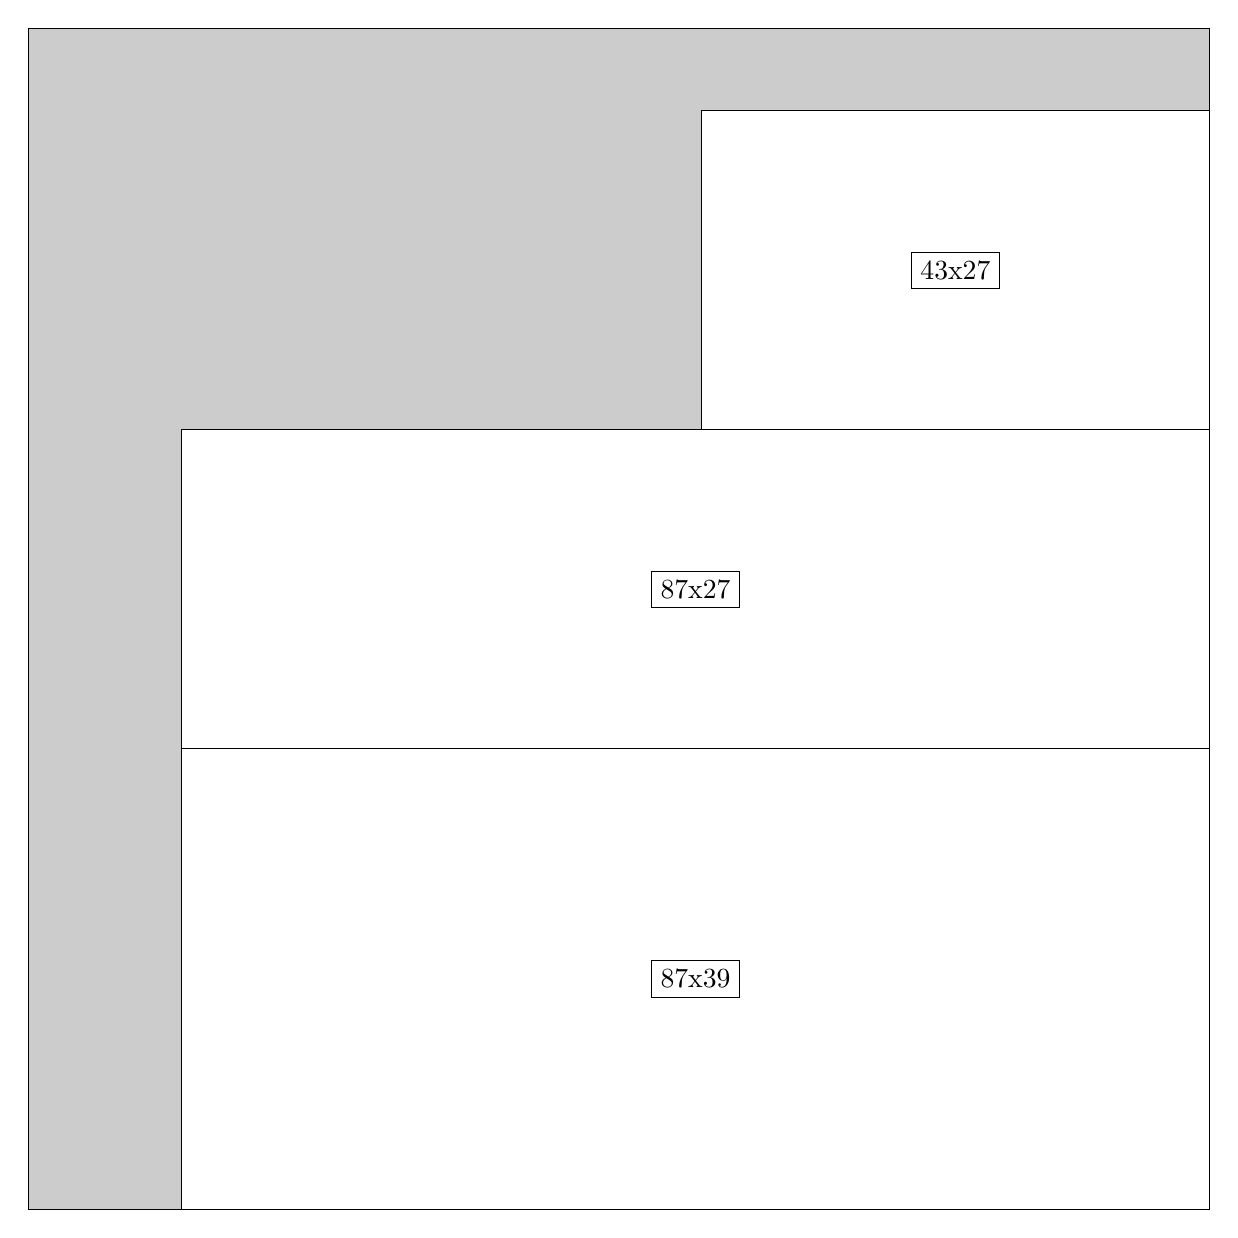
\begin{tikzpicture}[shorten >=1pt,scale=1.0,every node/.style={scale=1.0},->]
\tikzstyle{vertex}=[circle,fill=black!25,minimum size=14pt,inner sep=0pt]
\filldraw[fill=gray!40!white, draw=black] (0,0) rectangle (15.0,15.0);
\foreach \name/\x/\y/\w/\h in {87x39/1.95/0.0/13.049999999999999/5.85,87x27/1.95/5.85/13.049999999999999/4.05,43x27/8.549999999999999/9.9/6.45/4.05}
\filldraw[fill=white!40!white, draw=black] (\x,\y) rectangle node[draw] (\name) {\name} ++(\w,\h);
\end{tikzpicture}


w =87 , h =39 , x =13 , y =0 , v =3393
\par
w =87 , h =27 , x =13 , y =39 , v =2349
\par
w =43 , h =27 , x =57 , y =66 , v =1161
\par
\newpage


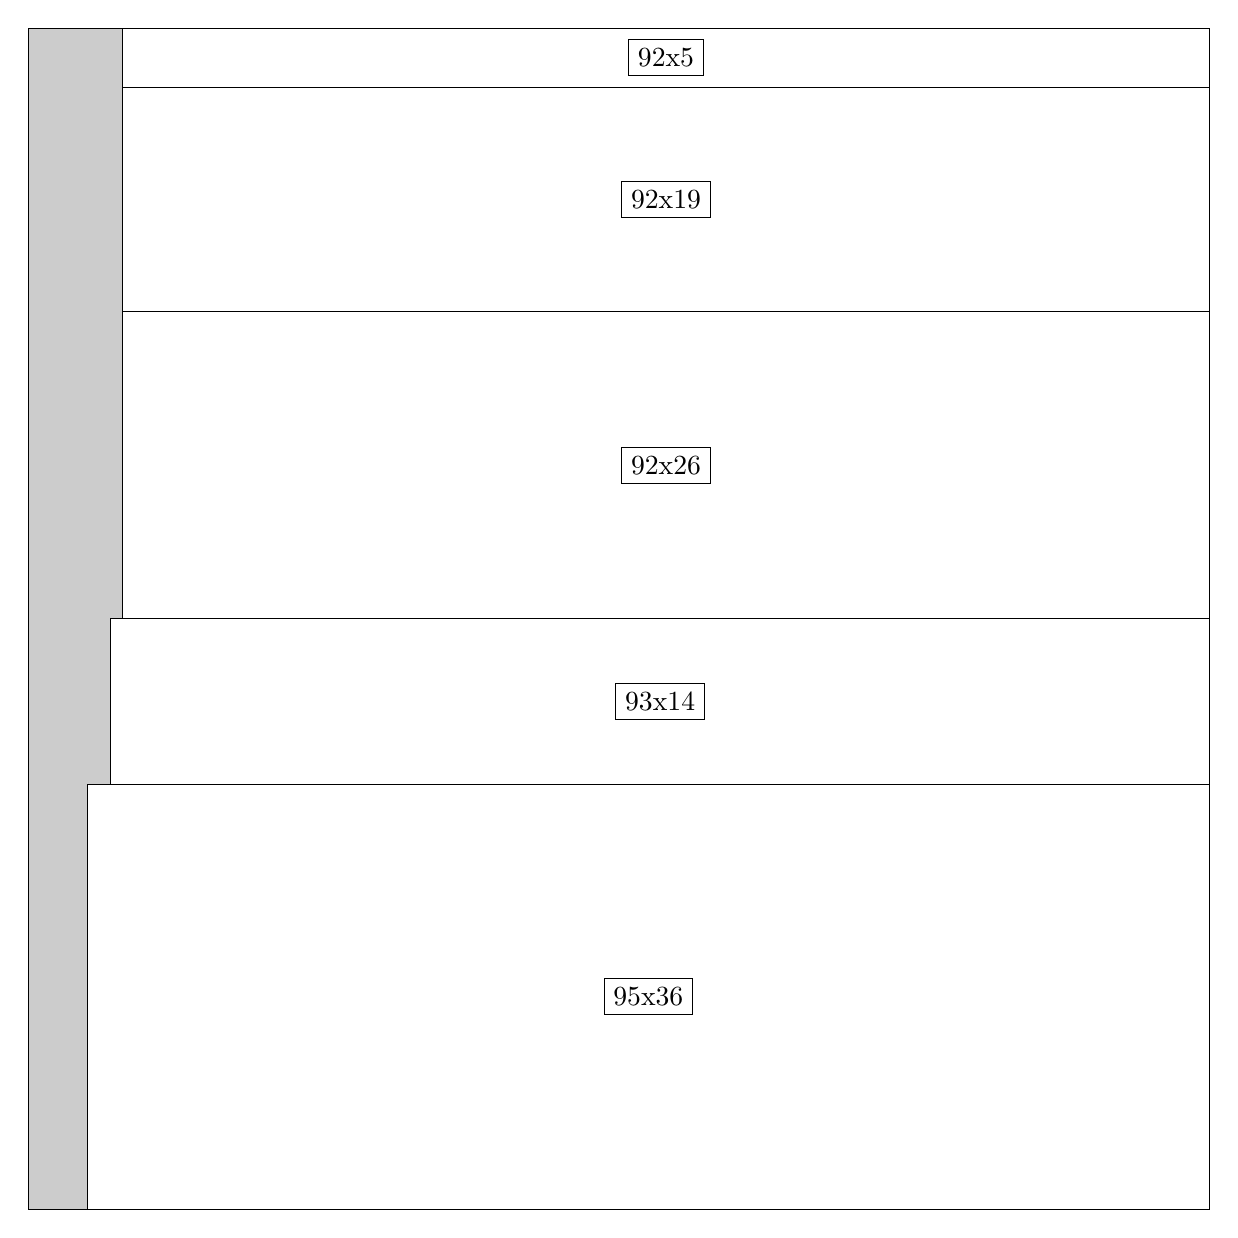
\begin{tikzpicture}[shorten >=1pt,scale=1.0,every node/.style={scale=1.0},->]
\tikzstyle{vertex}=[circle,fill=black!25,minimum size=14pt,inner sep=0pt]
\filldraw[fill=gray!40!white, draw=black] (0,0) rectangle (15.0,15.0);
\foreach \name/\x/\y/\w/\h in {95x36/0.75/0.0/14.25/5.3999999999999995,93x14/1.05/5.3999999999999995/13.95/2.1,92x26/1.2/7.5/13.799999999999999/3.9,92x19/1.2/11.4/13.799999999999999/2.85,92x5/1.2/14.25/13.799999999999999/0.75}
\filldraw[fill=white!40!white, draw=black] (\x,\y) rectangle node[draw] (\name) {\name} ++(\w,\h);
\end{tikzpicture}


w =95 , h =36 , x =5 , y =0 , v =3420
\par
w =93 , h =14 , x =7 , y =36 , v =1302
\par
w =92 , h =26 , x =8 , y =50 , v =2392
\par
w =92 , h =19 , x =8 , y =76 , v =1748
\par
w =92 , h =5 , x =8 , y =95 , v =460
\par
\newpage


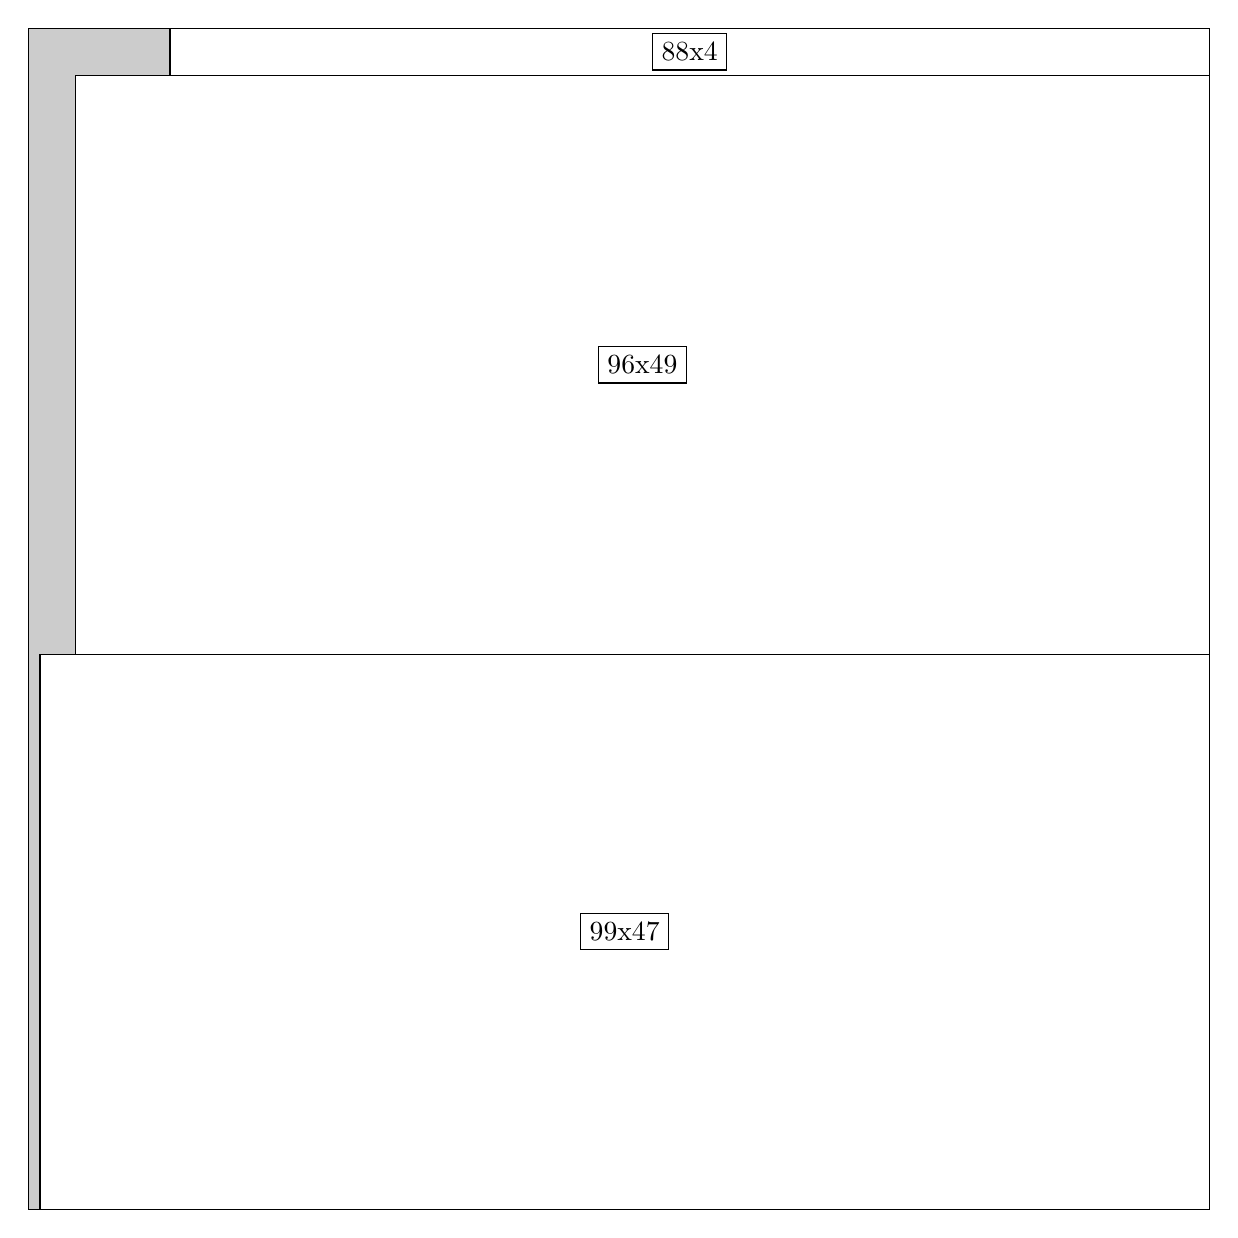
\begin{tikzpicture}[shorten >=1pt,scale=1.0,every node/.style={scale=1.0},->]
\tikzstyle{vertex}=[circle,fill=black!25,minimum size=14pt,inner sep=0pt]
\filldraw[fill=gray!40!white, draw=black] (0,0) rectangle (15.0,15.0);
\foreach \name/\x/\y/\w/\h in {99x47/0.15/0.0/14.85/7.05,96x49/0.6/7.05/14.399999999999999/7.35,88x4/1.7999999999999998/14.399999999999999/13.2/0.6}
\filldraw[fill=white!40!white, draw=black] (\x,\y) rectangle node[draw] (\name) {\name} ++(\w,\h);
\end{tikzpicture}


w =99 , h =47 , x =1 , y =0 , v =4653
\par
w =96 , h =49 , x =4 , y =47 , v =4704
\par
w =88 , h =4 , x =12 , y =96 , v =352
\par
\newpage


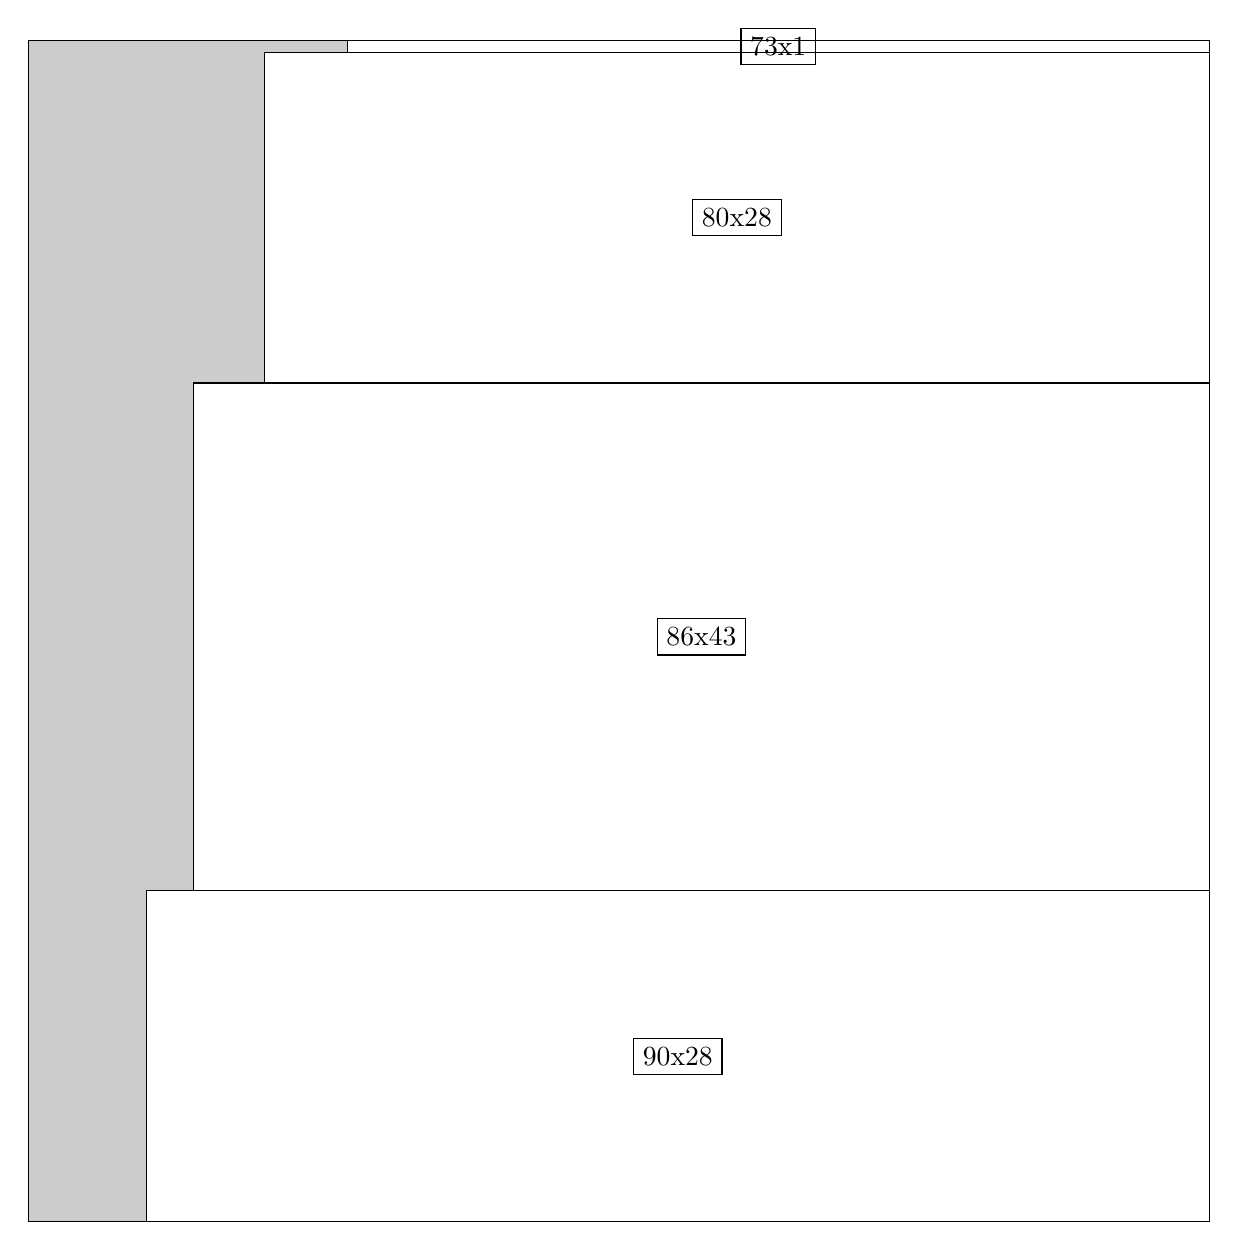
\begin{tikzpicture}[shorten >=1pt,scale=1.0,every node/.style={scale=1.0},->]
\tikzstyle{vertex}=[circle,fill=black!25,minimum size=14pt,inner sep=0pt]
\filldraw[fill=gray!40!white, draw=black] (0,0) rectangle (15.0,15.0);
\foreach \name/\x/\y/\w/\h in {90x28/1.5/0.0/13.5/4.2,86x43/2.1/4.2/12.9/6.45,80x28/3.0/10.65/12.0/4.2,73x1/4.05/14.85/10.95/0.15}
\filldraw[fill=white!40!white, draw=black] (\x,\y) rectangle node[draw] (\name) {\name} ++(\w,\h);
\end{tikzpicture}


w =90 , h =28 , x =10 , y =0 , v =2520
\par
w =86 , h =43 , x =14 , y =28 , v =3698
\par
w =80 , h =28 , x =20 , y =71 , v =2240
\par
w =73 , h =1 , x =27 , y =99 , v =73
\par
\newpage


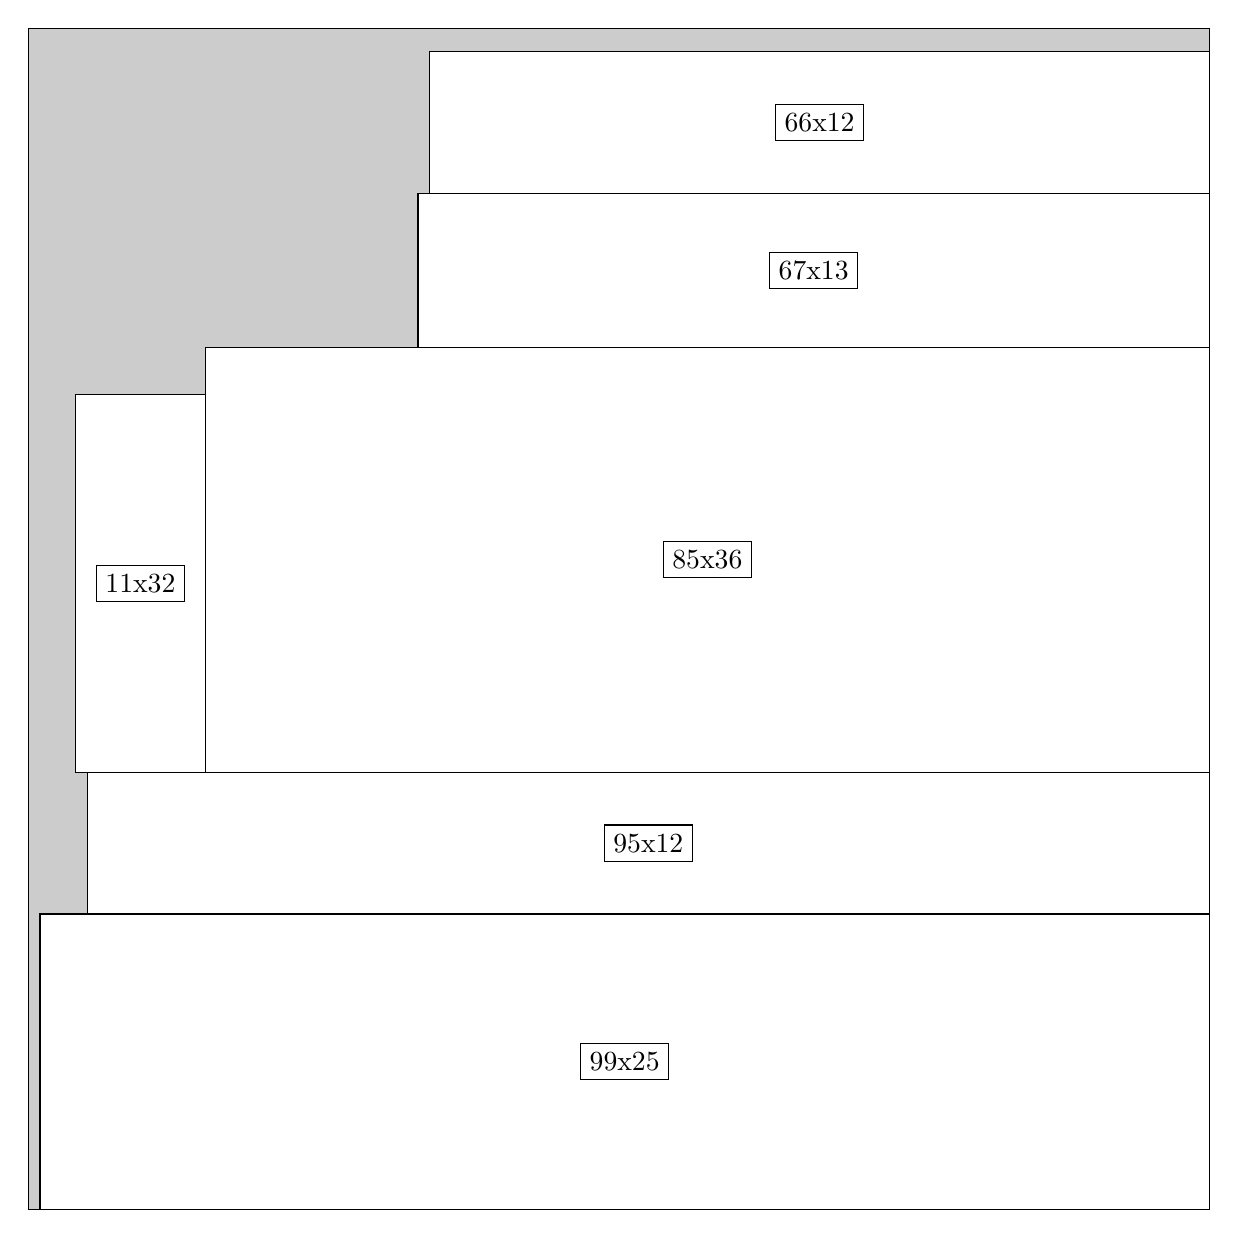
\begin{tikzpicture}[shorten >=1pt,scale=1.0,every node/.style={scale=1.0},->]
\tikzstyle{vertex}=[circle,fill=black!25,minimum size=14pt,inner sep=0pt]
\filldraw[fill=gray!40!white, draw=black] (0,0) rectangle (15.0,15.0);
\foreach \name/\x/\y/\w/\h in {99x25/0.15/0.0/14.85/3.75,95x12/0.75/3.75/14.25/1.7999999999999998,85x36/2.25/5.55/12.75/5.3999999999999995,11x32/0.6/5.55/1.65/4.8,67x13/4.95/10.95/10.049999999999999/1.95,66x12/5.1/12.9/9.9/1.7999999999999998}
\filldraw[fill=white!40!white, draw=black] (\x,\y) rectangle node[draw] (\name) {\name} ++(\w,\h);
\end{tikzpicture}


w =99 , h =25 , x =1 , y =0 , v =2475
\par
w =95 , h =12 , x =5 , y =25 , v =1140
\par
w =85 , h =36 , x =15 , y =37 , v =3060
\par
w =11 , h =32 , x =4 , y =37 , v =352
\par
w =67 , h =13 , x =33 , y =73 , v =871
\par
w =66 , h =12 , x =34 , y =86 , v =792
\par
\newpage


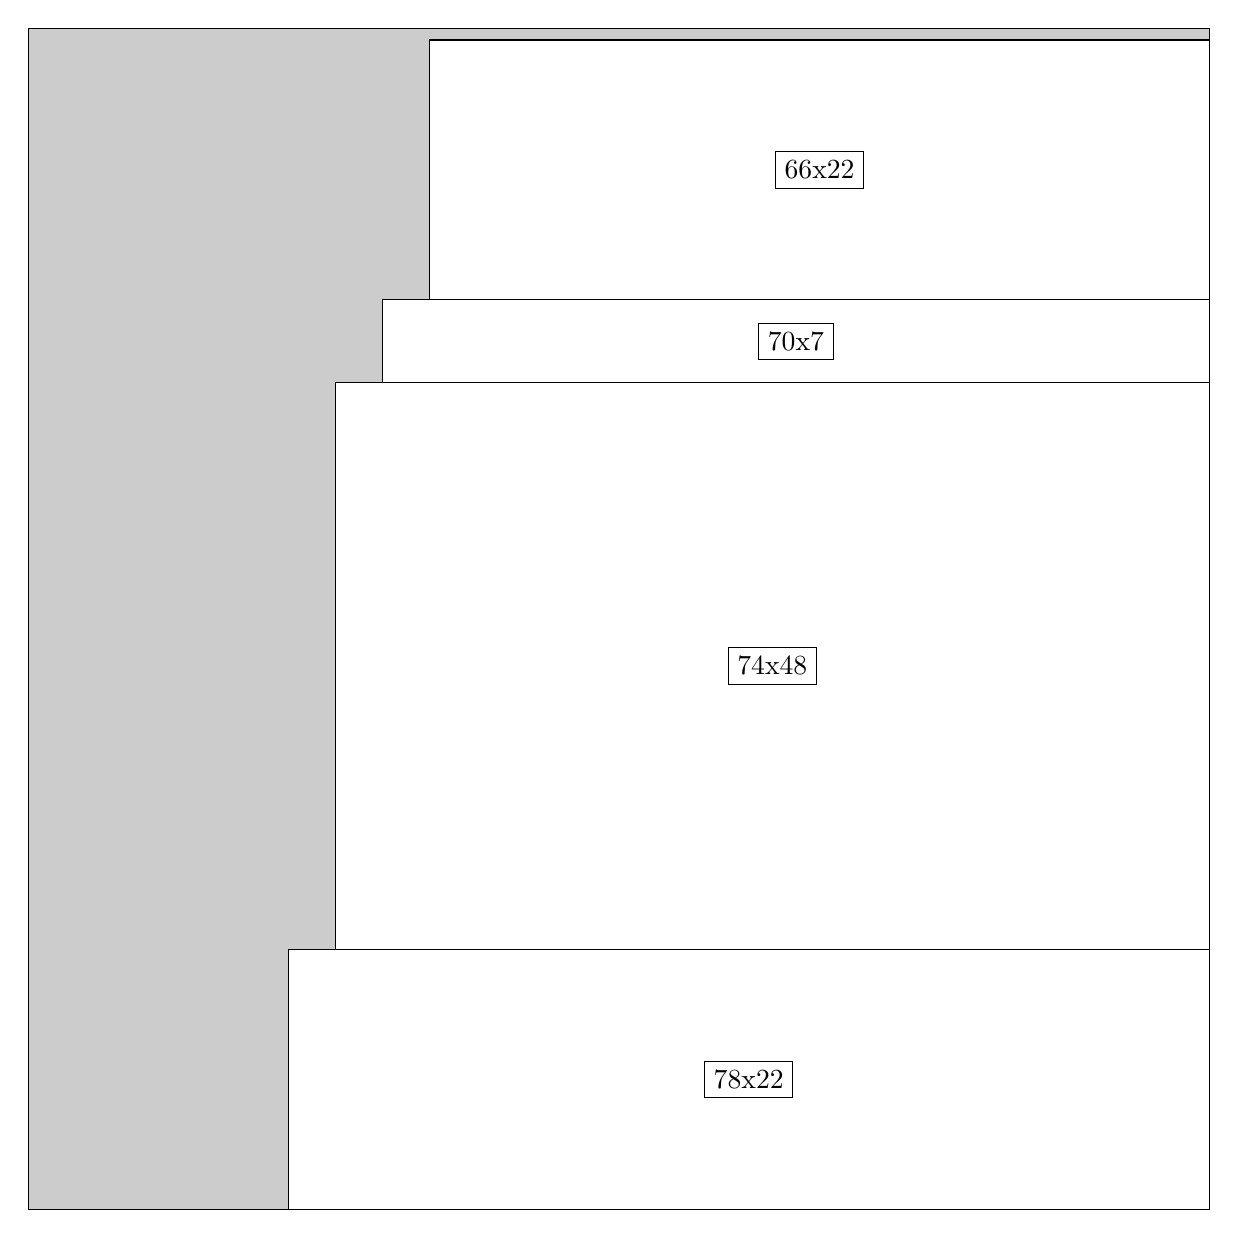
\begin{tikzpicture}[shorten >=1pt,scale=1.0,every node/.style={scale=1.0},->]
\tikzstyle{vertex}=[circle,fill=black!25,minimum size=14pt,inner sep=0pt]
\filldraw[fill=gray!40!white, draw=black] (0,0) rectangle (15.0,15.0);
\foreach \name/\x/\y/\w/\h in {78x22/3.3/0.0/11.7/3.3,74x48/3.9/3.3/11.1/7.199999999999999,70x7/4.5/10.5/10.5/1.05,66x22/5.1/11.549999999999999/9.9/3.3}
\filldraw[fill=white!40!white, draw=black] (\x,\y) rectangle node[draw] (\name) {\name} ++(\w,\h);
\end{tikzpicture}


w =78 , h =22 , x =22 , y =0 , v =1716
\par
w =74 , h =48 , x =26 , y =22 , v =3552
\par
w =70 , h =7 , x =30 , y =70 , v =490
\par
w =66 , h =22 , x =34 , y =77 , v =1452
\par
\newpage


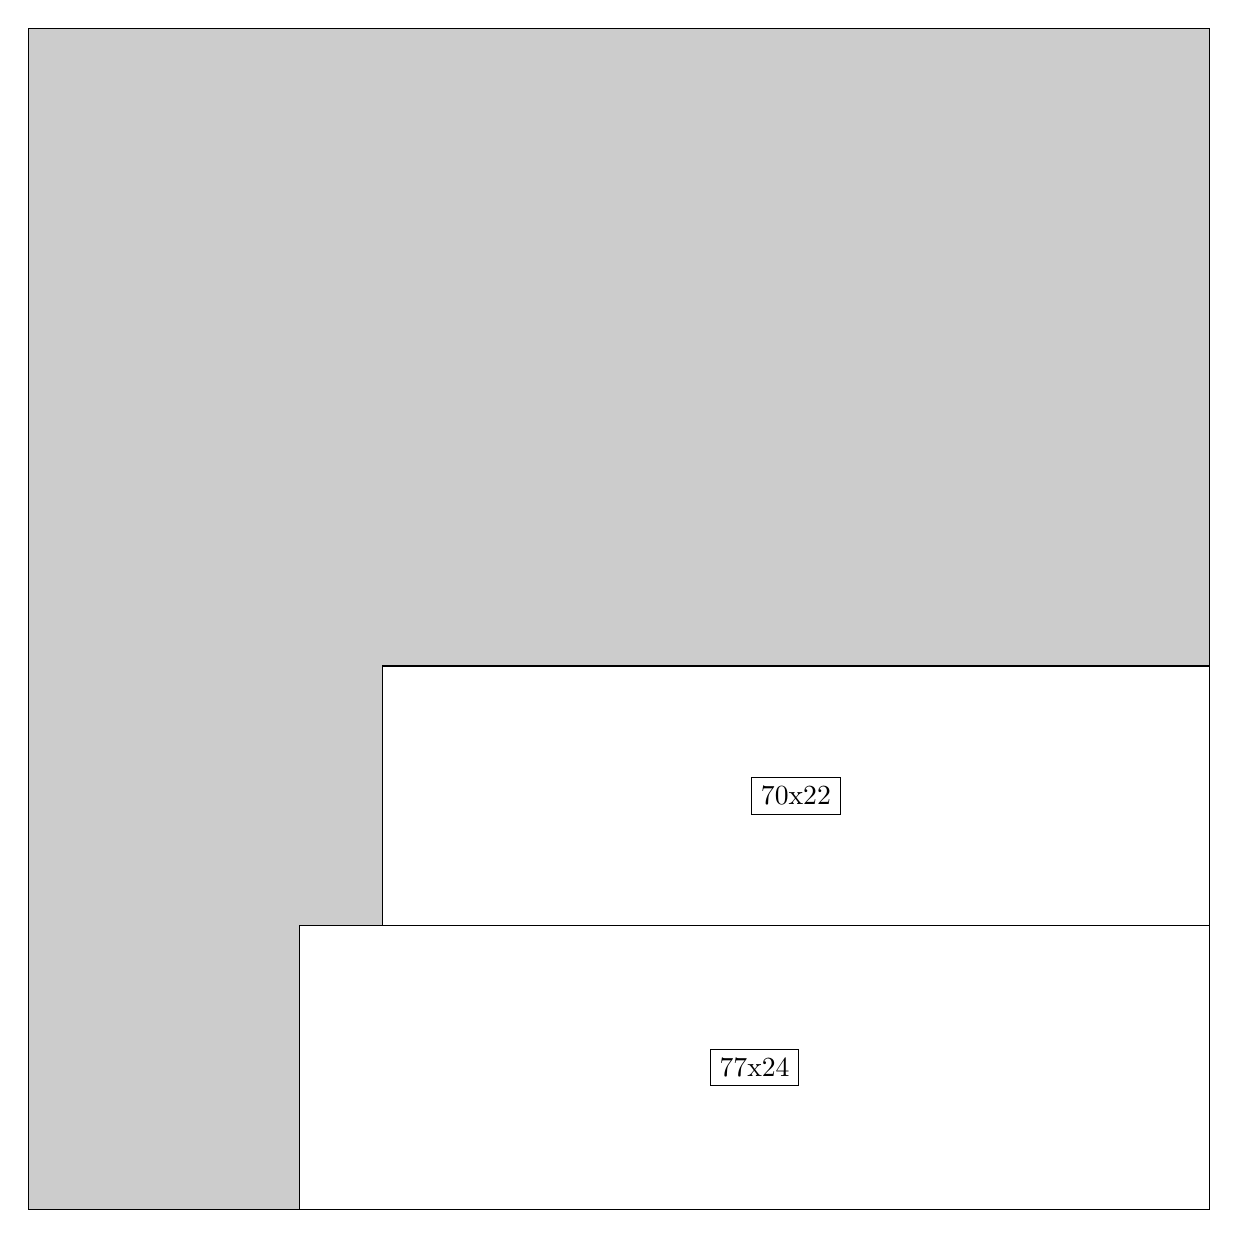
\begin{tikzpicture}[shorten >=1pt,scale=1.0,every node/.style={scale=1.0},->]
\tikzstyle{vertex}=[circle,fill=black!25,minimum size=14pt,inner sep=0pt]
\filldraw[fill=gray!40!white, draw=black] (0,0) rectangle (15.0,15.0);
\foreach \name/\x/\y/\w/\h in {77x24/3.4499999999999997/0.0/11.549999999999999/3.5999999999999996,70x22/4.5/3.5999999999999996/10.5/3.3}
\filldraw[fill=white!40!white, draw=black] (\x,\y) rectangle node[draw] (\name) {\name} ++(\w,\h);
\end{tikzpicture}


w =77 , h =24 , x =23 , y =0 , v =1848
\par
w =70 , h =22 , x =30 , y =24 , v =1540
\par
\newpage


\end{document}